%TCIDATA{LaTeXparent=0,0,relatorio.tex}
\ifx\compilewholereport\undefined
	\documentclass[11pt,a4paper,oneside]{book}
	
	% Escolher um dos seguintes formatos:
	\usepackage{ft2unb} % segue padrão de fontes do Latex
	
	% Pacotes
	\usepackage{graphicx}
	\usepackage{amsfonts}
	\usepackage{amsmath}
	\usepackage{amssymb}
	\usepackage[thmmarks,amsmath]{ntheorem}
	\usepackage{boxedminipage}
	\usepackage{theorem}
	\usepackage{fancybox}
	\usepackage{fancyhdr}
	\usepackage{url}
	\usepackage{afterpage}
	\usepackage{color}
	\usepackage{colortbl}
	\usepackage{rotating}
	\usepackage{makeidx}
	\usepackage{indentfirst}
	\usepackage{subcaption}
	\usepackage{todonotes}
	\usepackage{listings}
	\presetkeys{todonotes}{inline}{}
	
	\begin{document}
	\frontmatter
	\listoftodos
	\mainmatter
	
	%%%%%%%%%%%%%%%%%%%%%%%%%%%%
	%%%%%%%% Apagar coisas acima
	%%%%%%%%%%%%%%%%%%%%%%%%%%%%
\fi
\newcommand\dlq{\lq\lq{}}
\newcommand\drq{\rq\rq{}}

\lstdefinestyle{customVHDL}{
	  belowcaptionskip=1\baselineskip,
	  breaklines=true,
	  frame=l,
	  xleftmargin=\parindent,
	  language=VHDL,
	  showstringspaces=false,
	  basicstyle=\footnotesize\ttfamily,
	  keywordstyle=\itshape\color{blue!40!black},
	  commentstyle=\itshape\color{blue!40!black},
	  identifierstyle=\itshape\color{blue!40!black},
	  stringstyle=\itshape\color{blue!40!black},
}
                      
\chapter{Desenvolvimento}\label{CapDesenvolvimento}

\resumodocapitulo{Este capítulo trata da concepção dos experimentos realizados. Nele serão descritos com detalhes cada um dos experimentos, ficando a parte de análise reservada ao capítulo \ref{CapExperimentos}.}

\section{Introdu\c{c}\~{a}o}
%\vspace{0.8cm}
Devido ao caráter experimental e exploratório do objetivo proposto na seção \ref{sec:projeto}, decidiu-se dividir o projeto em vários experimentos menores.
Desta forma, além de garantir algum material mesmo que tudo dê errado, consegue-se simplificar o processo de pesquisa e desenvolvimento através dos pequenos passos e análises frequentes.

Como o objetivo final do projeto é a familiarização com as ferramentas e processos envolvidos na autoreconfiguração, decidiu-se começar estudando os elementos necessários para se realizar a reconfiguração dinâmica.
O passo seguinte mais lógico é o de estudar como funciona as memórias dos sistema e de que jeito elas seriam melhor utilizadas.
O último passo seria entender como funciona a autoreconfiguração em baixo nível, ou seja, como os dados devem ser entregues aos devidos componentes para que ela aconteça.
Para cada um destes experimentos foi proposto um teste que validasse o completo entendimento do mesmo.

\begin{figure}[h]
\centering
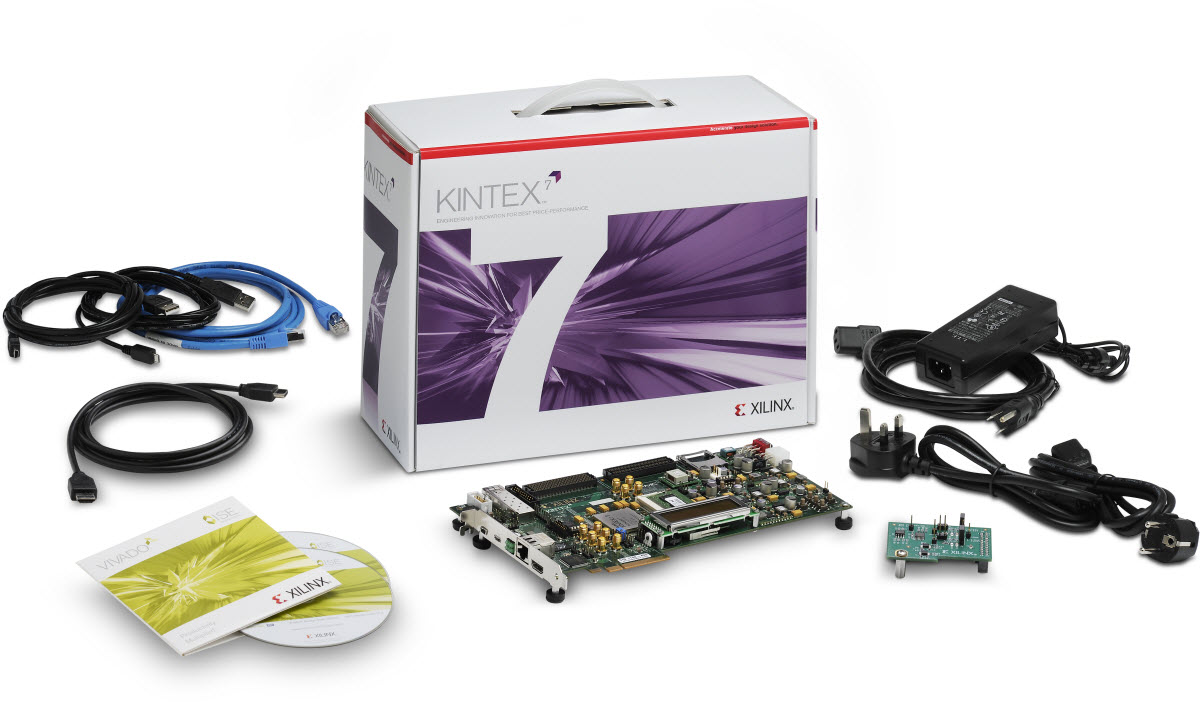
\includegraphics[width=0.5\textwidth]{figs/kintex-7_kc705}
\caption{Foto ilustrativa do kit de desenvolvimento Kintex-7 KC705 extraida do site da Xilinx.}
\label{fig:kc705}
\end{figure}

Para o desenvolvimento desse projeto, escolheu-se utilizar o kit de desenvolvimento da Xilinx\textregistered{} chamado Kintex-7 KC705.
O único critério utilizado foi a disponibilidade dos equipamentos no início do projeto e a capacidade do dispositivo de realizar a reconfiguração parcial dinâmica.
Este kit possui FPGA modelo XC7K325T-2FFG900C, leitor de cartão de memória, conector PCIe\textregistered{}, memória DDR3, visor de 7-segmentos e porta ethernet, dentre outros.

Escolheu-se ainda, de forma arbitrária, o uso da linguagem VHDL para a descrição de \textit{hardware} ao invés da Verilog.

\section{Experimento 1 - Reconfiguração Dinâmica}
De forma a dar validade a todo o projeto, foi preciso desenvolver um experimento para se entender o processo de desenvolvimento de sistemas reconfiguráveis dinamicamente e algumas peculiaridades do kit de desenvolvimento.

\subsection{Fluxo de Ferramentas}
A primeira coisa que se destaca no desenvolvimento de dispositivos dinamicamente reconfiguráveis é a diferença no fluxo de ferramentas, também conhecido como \textit{software tools flow}, em relação ao fluxo tradicional \cite{ug743}.
Esta diferença é motivada pela necessidade de construção de diversos \textit{bitfiles} parciais.
Como pode-se ver da figura \ref{fig:softwareflow}, o fluxo tradicional requer apenas o uso do programa ISE, e opcionalmente do XPS e do SDK, para a construção de um projeto de \textit{hardware} e o iMPACT para a programação da FPGA.
No fluxo para reconfiguração dinâmica mostrado na figura \ref{fig:prsoftwareflow}, além das ferramentas do fluxo tradicional, faz-se necessário o uso da ferramenta XST para a síntese do \textit{netlist} e do PlanAhead para a definição de partições e configurações.
Note que estes fluxos não apresentam as únicas opções de fluxo de ferramentas, mas as que foram utilizadas neste projeto.

\begin{figure}[h]
	\centering
       	\begin{subfigure}[b]{\textwidth}
       		\centering
		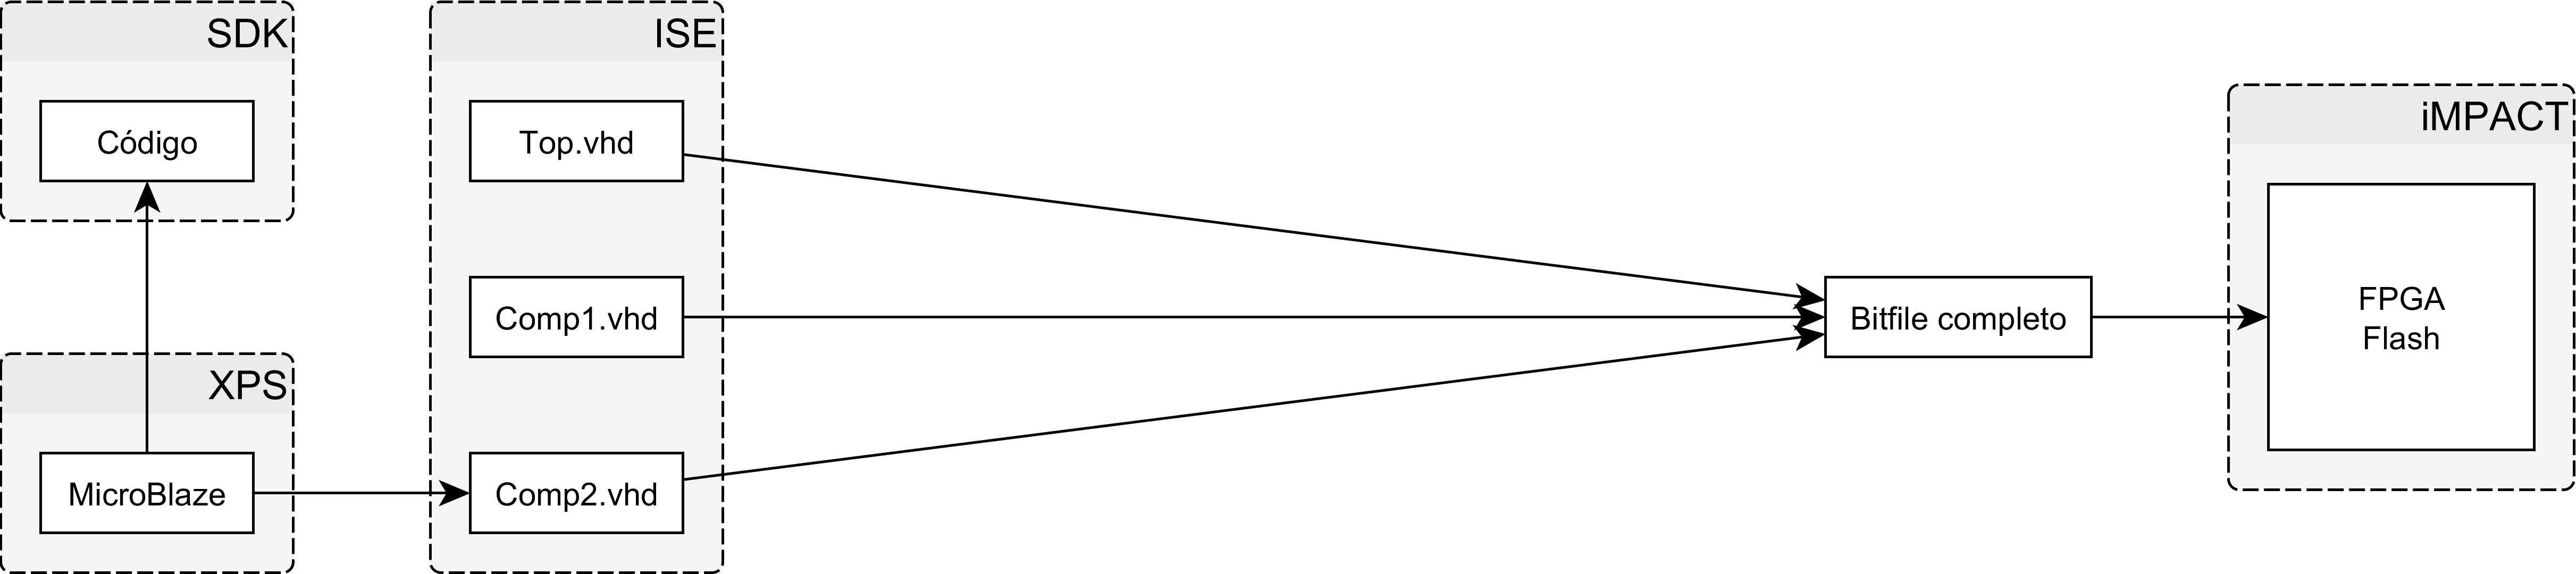
\includegraphics[height=100px]{figs/ex1/softwareflow}
		\caption{Foto ilustrativa do \textit{software-flow} tradicional. Note que o uso do microcontrolador MicroBlaze é opcional, tornando os primeiros blocos, SDK e XPS, também opcionais.}
		\label{fig:softwareflow}
	\end{subfigure}\\
	\begin{subfigure}[b]{\textwidth}
		\centering
		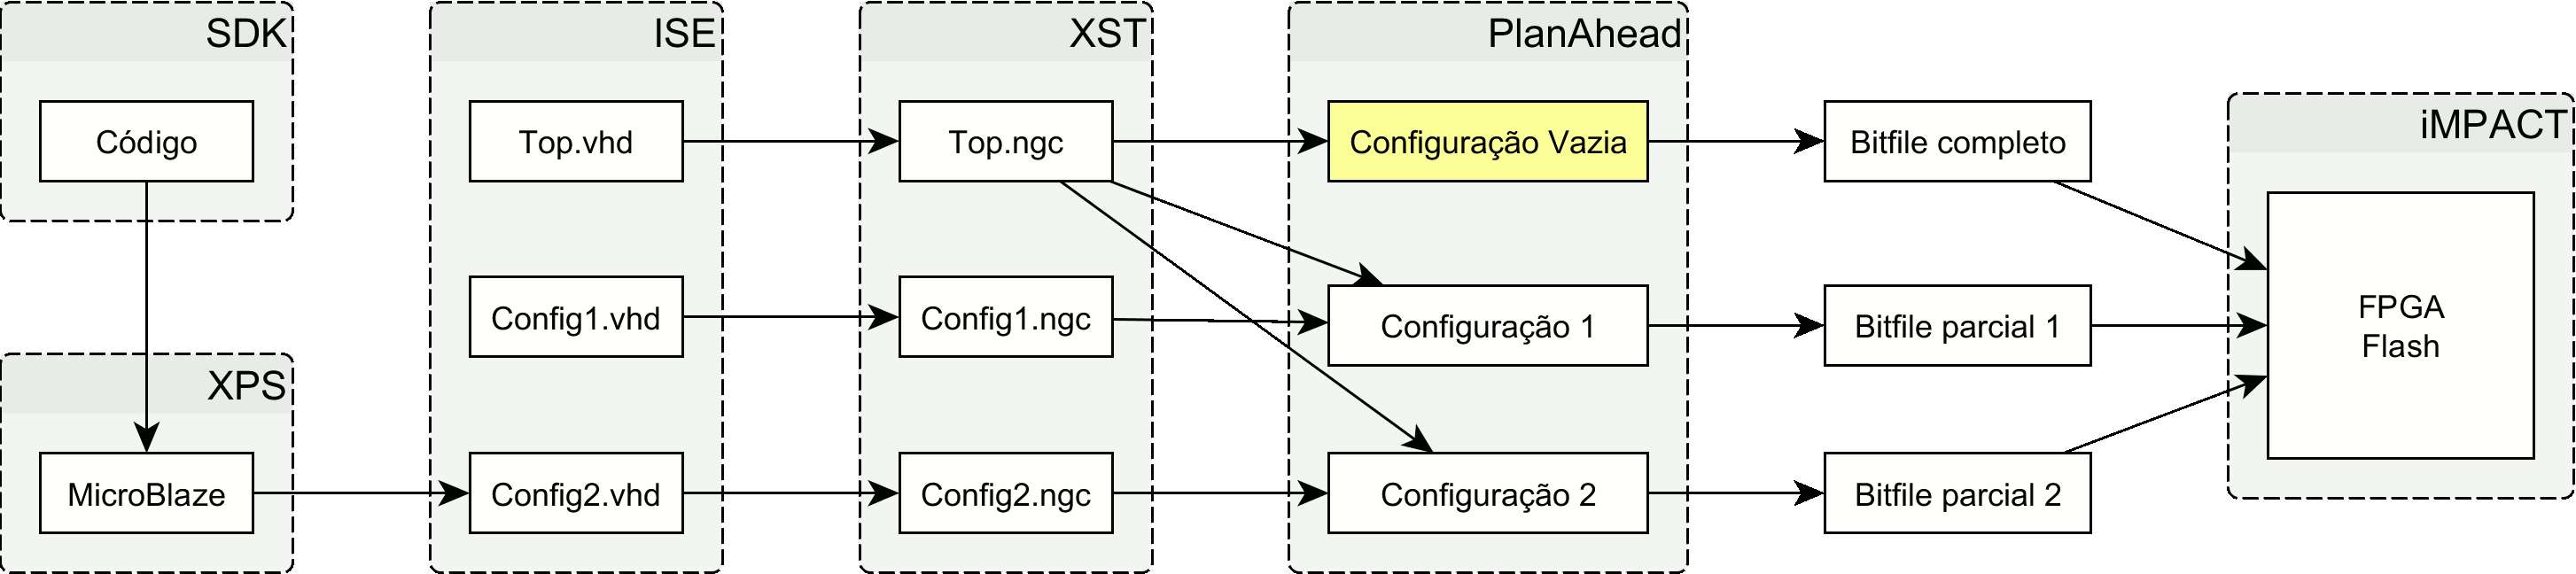
\includegraphics[height=100px]{figs/ex1/prsoftwareflow}
		\caption{Foto ilustrativa do \textit{software-flow} para a reconfiguração dinâmica. Assim como no caso tradicional, o uso do SDK e do XPS são opcionais. Note que o bloco em amarelo indica a configuração padrão, que será programada inicialmente. A escolha da configuração padrão é arbitrária.}
		\label{fig:prsoftwareflow}
	\end{subfigure}
	\caption{Comparação dos fluxos de ferramentas. Note que estes fluxos não apresentam as únicas opções de fluxo de ferramentas, mas as que foram utilizadas neste projeto.}
	\label{fig:softwareflow:comparacao}
\end{figure}

Reconfiguração parcial pede uma síntese utilizando o método \dlq de baixo para cima\drq{} (\textit{bottom-up}), mas uma implementação \dlq de cima para baixo\drq{} (\textit{top-down}) \cite{ug743}, ou seja, a implementação acontece construindo primeiro a interface com o sistema e depois os componentes auxiliares, mas a síntese precisa ser realizada no sentido oposto.
Esta implementação é equivalente a se construir diversos projetos tradicionais com alguma lógica em comum, onde a síntese deve garantir que esta lógica em comum seja implementada da mesma forma para as diferentes configurações \cite{ug702}.

\subsection{Peculiaridades}
O kit de desenvolvimento utilizada apresenta algumas peculiaridades com relação aos kits comuns.
A seguir serão apresentadas algumas destas peculiaridades.

\subsubsection{Relógios}
Diferentemente das FPGAs comuns, a que está presente neste kit contém um relógio diferencial, ou seja, dois sinais compoem tal relógio.
A razão para tal é a presença de circuitos sensíveis a interferência, tais como \textit{transceivers}, que são muito menores em sinais diferenciais.
O kit disponibiliza duas opções de relógio: o SYSCLK e o USER\_CLOCK.
O primeiro possui uma frequência fixa de oscilação de 200 MHz.
O segundo possui uma frequência original de 156.250 MHz, mas pode ser programado através de uma interface I$^2$C para ter frequências entre 10 MHz e 810 MHz.
Por motivos de simplicidade, utilizou-se o SYSCLK.
Para poder se trabalhar com o sinal diferencial, construiu-se, utilizando as ferramentas do ISE, um componente para tratamento do sinal de relógio.
Este componente recebe o sinal diferencial, reduz sua frequência para 20 MHz, que corresponde ao menor valor suportado pelas PLLs da placa, e emite um sinal convencional.

\subsection{Teste}
Para se entender mais a fundo o fluxo de projeto, nada melhor que construir um projeto.
Para isso, implementou-se o sistema esquematizado na figura \ref{fig:ex1:componentes}.
Este sistema contém o \dlq{}Top\drq{} para interfaceamento com a FPGA, o \dlq{}Clocks\drq{} para tratamento do sinal de relógio, a \dlq{}Static\drq{}, que possui um lógica estática para demonstrar que a reconfiguração de uma partição não interfere com outra, e a \dlq{}Dynamic\drq{}, que possui a lógica a ser alterada dinâmicamente.

\begin{figure}[h]
\centering
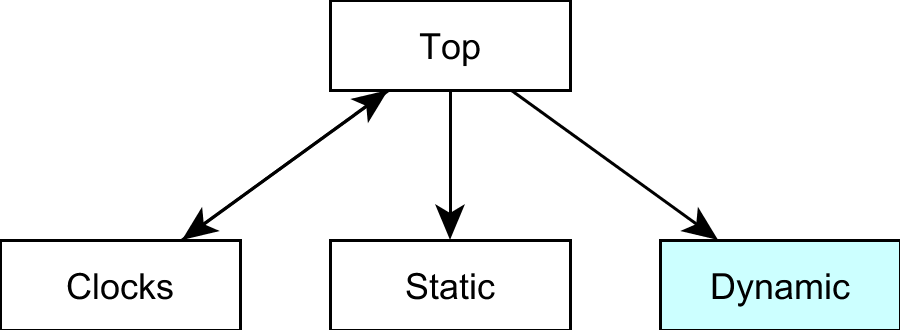
\includegraphics[width=0.5\textwidth]{figs/ex1/componentes}
\caption{Foto ilustrativa do sistema desenvolvido para o teste de validação do experimento 1. Ele é composto por uma parte estática e uma parte dinâmica. O elementos em branco são estáticos e os em azul são dinâmicos.}
\label{fig:ex1:componentes}
\end{figure}

\paragraph{Estrutura de Pastas}
A questão da organização do projeto em pastas bem específicas é sempre bem mencionado na literatura \cite{ug702, ug743, ug744}.
Os manuais recomendam a seguinte estrutura de pastas.
\begin{lstlisting}
Projeto/
  Source/           //codigos-fonte organizados segundo particao
  Implementation/   //contem pastas para cada config. dinamica gerada
  Synth/            //contem pastas com os arquivos .xst e .prj
  Tools/            //ferramentas para automacao da sintese
  PlanAhead/        //pasta para o projeto do PlanAhead
\end{lstlisting}
Esta estrutura de pastas foi obedecida por ajudar a manter o ambiente de desenvolvimento limpo.

\subsubsection{Comportamento}
Como explicado anteriormente, o projeto de um sistema parcialmente reconfigurável pode ser visto como vários projetos completos com partes em comum.
Seguindo essa lógica, dois projetos com comportamentos diferentes foram construídos usando como base a figura \ref{fig:ex1:componentes}.
O comportamento individual de cada módulo ou componente será descrito a seguir.
Este passo está ilustrado no fluxo de ferramentas da figura \ref{fig:prsoftwareflow} como ISE.

O componente \dlq{}Static\drq{} possui uma entrada para um relógio pulsando a 2 Hz e uma saída para um LED.
Seu comportamento apenas faz com que o LED pisque a uma frequência de 2 Hz, o que permite observar seu funcionamento durante a reconfiguração do componente \dlq{}Dynamic\drq{}.

O componente \dlq{}Dynamic\drq{} possui dois comportamentos distintos.
O primeiro deles é o de um simples contador crescente de 4 bits.
O segundo é uma máquina de estados que alterna os 4 bits de saída entre "1100" e "0011" a cada pulso de relógio.
Este componente possui uma entrada para um relógio pulsando a 1 Hz e uma palavra de 4 bits de saída.
A frequência de operação deste componente foi escolhida para ser a metade da frequência da \dlq{}Static\drq{} para poder ser visualmente comprovado que \dlq{}Static\drq{} não para de funcionar quando \dlq{}Dynamic\drq{} está sendo reconfigurado.

O componente \dlq{}Clocks\drq{} recebe os sinais diferenciais de relógio e o transformam em um sinal comum.
O bloco lógico utilizado para isso foi construído usando ferramentas presentes no ISE.
Uma vez que a ferramenta permitia a construção de um relógio com divisor de frequência, a frequência do relógio da placa, que nesse caso é de 200 MHz, foi reduzida para 20 MHz.

O módulo \dlq{}Top\drq{} instancia os componentes descritos acima e faz a interface dos mesmos com a FPGA.
O componente dinâmico precisa de uma declaração de protótipo para ser instanciado corretamente.
Utilizou-se o código abaixo para esta finalidade.
\begin{lstlisting}[style=customVHDL]
component dynamic
    port ( clk  : in  std_logic;
           leds : out std_logic_vector (3 downto 0));
end component;
\end{lstlisting}
O módulo \dlq{}Top\drq{} possui também um divisor de frequência para reduzir a frequência devolvida por \dlq{}Clocks\drq{} para 1 e 2 Hz.

\subsubsection{Síntese}
Com o comportamento do projeto definido, o próximo passo segundo o fluxo de ferramentas é a síntese.
Este passo é necessário uma vez que o próximo passo, referente ao PlanAhead, não aceita como entrada códigos-fonte.
Os códigos-fonte precisam passar por uma etapa de síntese separada para poderem ser importados no PlanAhead.
Este passo está ilustrado no fluxo de ferramentas da figura \ref{fig:prsoftwareflow} como XST.

O comando XST recebe tipicamente um \textit{script} contendo o endereço dos códigos-fonte, o nome do arquivo de saída, o tipo do arquivo de saida, o modelo da FPGA utilizada e uma indicação do código-fonte principal.
O comando para iniciar o processo é o seguinte.
\begin{lstlisting}[style=customVHDL]
xst.exe -ifn Top.xst
\end{lstlisting}
O arquivo \dlq{}Top.xst\drq{} contém os seguintes comandos.
\begin{lstlisting}[style=customVHDL]
run
-ifn Top.prj
-ofn Top
-ofmt NGC
-p xc7k325t-2-ffg900
-top top
\end{lstlisting}
O arquivo \dlq{}Top.prj\drq{} contém os endereços dos arquivos, conforme a seguir.
\begin{lstlisting}[style=customVHDL]
vhdl work "../../Sources/static/top.vhd"
vhdl work "../../Sources/static/static.vhd"
vhdl work "../../Sources/static/clocks.vhd"
\end{lstlisting}\

Note que estes comandos e arquivos indicados acima são para síntese dos componentes estáticos.
Uma vez que não existe nenhuma restrição especial para tais componentes, eles podem ser síntetizados para um único arquivo de saída.
O mesmo não pode ser dito para os elementos dinâmicos.
Cada componente dinâmico precisa ser sintetizado em separado para depois ser incluído no projeto através do PlanAhead.

A síntese de componentes dinâmicos precisa ser realizada com um \textit{script} \dlq{}.xst\drq{} ligeiramente diferente.
Como mostrado a seguir, faz-se necessária a inclusão do argumento \dlq{}-iobuf NO\drq{}, que desabilita a inserção de componentes de Entrada/Saída \cite{ug743, ug748}.
\begin{lstlisting}[style=customVHDL]
run
-ifn DynFSM.prj
-ofn DynFSM
-ofmt NGC
-p xc7k325t-2-ffg900
-top dynamic
-iobuf NO
\end{lstlisting}
Note que o arquivo \dlq{}DynFSM.prj\drq{} contém informações sobre o cógigo-fonte do componente dinâmico, como mostrado a seguir.
\begin{lstlisting}[style=customVHDL]
vhdl work "../../Sources/dynamic_fsm/dynamic.vhd"
\end{lstlisting}

Existe também a possibilidade de construção de um \textit{script} para a síntese automática de todos os arquivos.
Utilizou-se aqui uma adaptação do arquivo em linguagem TCL usado pela Xilinx em seus manuais \cite{ug702, ug743, ug744}.
A única coisa que se faz neste \textit{script} é a construção dinâmica dos comandos com base em listas de arquivos pré-informados.

\subsection{PlanAhead}
Com os arquivos síntetisados, pode-se começar a etapa referente ao PlanAhead.
Nela, importaremos os arquivos da etapa anterior, criaremos a partição reconfigurável, mapearemos esta partição no dispositivo, criaremos configurações alternativas, promoremos tais configurações e geraremos os \textit{bitfiles} para a programação do dispositivo.

\todo{Promoção de partições explicado em ug748, p. 50.}

\subsection{iMPACT}

\todo{Explicar como fui para o próximo experimento}
\section{Experimento 2 - Teste de Acesso a Memória}
\todo{Descrever o experimento 2}
\todo{Descrever os tipos de memória disponíveis e o porque de escolher a DDR3}
\todo{Explicar porque não deu certo e como fui para o próximo experimento}
\section{Experimento 3 - Teste do \textit{Bootloader}}
\todo{Descrever o experimento 3}
\todo{Explicar como fui para o próximo experimento}
\section{Experimento 4 - Teste da Autoreconfiguração com \textit{Bootloader} Dedicado}
\todo{Descrever o experimento 4}
\todo{Explicar como fui para o próximo experimento}
\section{Experimento 5 - Teste da Autoreconfiguração}
\todo{Descrever o experimento 5}
\todo{Explicar como fui para o próximo experimento}

\ifx\compilewholereport\undefined
	\bibliographystyle{plain} 
	%\bibliography{bibliografia.bib}
	\newsavebox\mytempbib\savebox\mytempbib{\parbox{\textwidth}{\bibliography{bibliografia}}}

	\end{document}
\fi